\chapter[Genetika]{Genetika}
\label{genetika} % id kapitoly pre prikaz ref

Genetika

\section{Molekulárne základy dedičnosti ALMOST DONE}

Status: almost DONE
Source: Prednášky 9, 10, (11?), 12, 13, 14\\
\\
štruktúra a replikácia DNA, transkripcia, translácia, regulácia génovej expresie na transkripčnej a post-transkripčnej úrovni. \\
\subsection*{Štruktúra DNA}
DNA\\
\tab báza (C, T, U - pyrimidín, A, G - purín) \\
\tab Deoxyribóza\\
\tab Fosfát\\
\tab Dvojvláknová, helikálna, antiparalelná\\
\tab -$PO_3^-$ koniec -- 5` fosfátový\\\\
\tab -OH koniec -- 3` ribózový/deoxyribózový\\
\tab Vodíkové väzby\\
\\
%Obr $\rightarrow$ prezent 9, slide 23
\includegraphics[width=0.5\textwidth, page=23]{materials/Genetika/prednasky-genetika/09_DNA_a_jej_uloha_v_dedicnosti.pdf}
\\
RNA\\
\tab U + ribóza, 1 vlákno\\
\\
\subsection*{Replikácia}
\tab Semikonzervatívna -- jedno templátové vlákno z pôvodnej + 1 nové\\
\tab Rozdelenie DNA --helikáza, energia z hyrdolýzy ATP\\
\tab \tab SSB single strand binding proteíny zabraňujú spojeniu\\
\tab Nové vlákno vzniká 5` $\rightarrow$ 3`\\
\tab DNA polymerázy replikujú\\
\tab \tab Potrebujú na začatie RNA primer, ktorý pridá DNA primáza\\
\tab Replikačná vidlica -- Replikácia ide od “stredu” (origin) -- oboma smermi naraz\\
\tab Leading a Lagging strand\\
\tab \tab Keďže syntéza ide 5`$\rightarrow$ 3`, lagging strand sa syntetizuje po úsekoch -- okazakiho fragmenty\\
\tab \tab Lagging strand -- DNA polymeráza 3 syntetizuje, DNA polymeráza 1 odstraňuje RNA primery a nahrádza ich DNA a  DNA ligáza opravuje medzery, kde sa nadpájajú fragmenty\\
\tab \tab Lagging strand zle replikuje teloméry -- enzým telomeráza ich predlžuje (obsahuje RNA a proteínovú časť, podľa tej RNA sa dosyntetizuje telomér)\\
\subsection*{Oprava DNA}
Transpozón -- úsek DNA, schopný meniť miesto v genóme\\
\subsection*{Transkripcia, translácia, syntéza bielkovín}
Centrálna dogma -- smer toku informácií\\

%Obrázok prezent 12, slide 23\\
\includegraphics[width=0.5\textwidth, page=23]{materials/Genetika/prednasky-genetika/12_Od_DNA_k_RNA.pdf}
\\
DNA $\rightarrow$ Transkripcia $\rightarrow$ mRNA $\rightarrow$ translácia $\rightarrow$ proteín\\
Kódujúce vlákno + Templátové vlákno (komplementárne ku kódujúcemu) $\rightarrow$ mRNA vlákno (rovnaké ako kódujúce, ale T $\rightarrow$ U)\\
Iniciácia -- RNA polymeráza + sigma faktor dosadnú\\
Elongácia -- predlžovanie RNA vlákna\\
Terminácia -- $\rho$ proteín $\rightarrow$ nascentné vlákno RNA,  alebo bez neho $\rightarrow$ zloženie RNA do 2D štruktúry\\
\\
\tab U eukaryotov\\
\tab \tab Intrón + Exón $\rightarrow$ transkripcia $\rightarrow$ pre-mRNA $\rightarrow$ splicing, processing $\rightarrow$ mRNA $\rightarrow$ transport, čiapočka, poly(A) chvost $\rightarrow$ translácia $\rightarrow$ proteín\\
\tab \tab Obrázok prezent 12 slide 34\\
\tab \tab 3 RNA polymerázy miesto 1\\
\tab \tab \tab rRNA\\
\tab \tab \tab pre-mRNA\\
\tab \tab \tab tRNA, 5S rRNA, malé jadrové RNA\\
\\
\tab mRNA, rRNA -- zložka ribozómov, tRNA -- prenáša AK\\
\tab Malé RNA -- miRNA, shRNA, siRNA -- sa podieľajú na génovej expresii\\
\tab Začiatok transkripcie RNA polymerázou 2 potrebuje bazálny iniciačný komplex (TATA box + stuff)\\
\tab Post-transkripčné úpravy\\
\tab \tab CAP, poly(A) chvost\\
\tab \tab Možná deaminácia\\
\tab \tab Alternatívny splicing intrónov $\rightarrow$ rôzne proteíny (12, 52)\\
\tab \tab Trans-splicing -- kombinácia exónov z rôznych génov\\
\subsection*{Translácia}
\tab Skladanie ribozómov: proteíny $\rightarrow$ rRNAs $\rightarrow$ ribozóm. Syntéza rRNA v jadierku\\
\tab tRNA: \tab antikodón tRNA ~ kodón mRNA\\
\tab \tab AK sú pripojené na 3` koniec tRNA\\
\tab \tab Aj modifikované nukleotidy\\
\tab \tab Iniciácia proteosyntézy, Elongácia polypeptidu, terminácia translácie\\
\tab 3 binding sites v ribozóme (E-exit, P-peptidyl, A-aminoacyl)\\
\tab 5` $\rightarrow$ 3`\\
\tab Wobble pozícia -- Inozín -- môže tvoriť pár s viac bázami\\
\subsection*{Regulácia génovej expresie}
\tab Prezentácia 14 TODO\\

\section{Cytologické základy dedičnosti}
\subsection*{štruktúra chromozómov na mikroskopickej a molekulovej úrovni}
\subsection*{funkcia chromozómov}
\subsection*{distribúcia genetických štruktúr pri delení buniek eukaryotov (mitóza a meióza)}
\subsection*{Spôsoby rozmnožovania organizmov a ich úloha v udržiavaní genetickej variability}

\section{Mendelistická dedičnosť}
\subsection*{monohybridné, dihybridné a polyhybridné kríženie s úplnou dominanciou}
\subsection*{princípy a možnosti genetickej analýzy u človeka}

\section{Rozšírená mendelistická genetická analýza}
\subsection*{neúplná dominancia a kodominancia}
\subsection*{mnohonásobný alelizmus}
\subsection*{letálne gény}
\subsection*{interakcie génov}
\subsection*{penetrancia a expresivita}

\section{Dedičnosť a pohlavie}
\subsection*{genetická determinácia pohlavia u mikroorganizmov, rastlín, živočíchov a človeka}
\subsection*{štruktúra a funkcia pohlavných chromozómov}
\subsection*{dedičnosť znakov, ktorých gény sú uložené na pohlavných chromozómoch (dedičnosť znakov viazaných na pohlavie)}
\subsection*{dedičnosť znakov pohlavím ovládaných a ovplyvnených}

\section{Väzba génov}
\subsection*{väzbové skupiny}
\subsection*{priebeh dedičnosti znakov pri väzbe génov (úplnej a neúplnej)}
\subsection*{väzbové fázy}
\subsection*{techniky mapovania génov}
\subsection*{“trojbodový test” (kríženie trihybrida s homozygotne recesívnym rodičom)}
\subsection*{interferencia a koincidencia}

\section{Mimojadrová dedičnosť}
\subsection*{štruktúra a funkcia mitochondriálneho a chloroplastového genómu}
\subsection*{genetický kód v DNA mitochondrií}
\subsection*{dedičnosť znakov determinovaných mimojadrovými genómami}
\subsection*{charakteristické znaky mimojadrovej dedičnosti}
\subsection*{symbionty a ich úloha v mimojadrovej dedičnosti}
\subsection*{matroklinný efekt}

\section{Genetická analýza u prokaryotov}
\subsection*{štruktúra chromozómu}
\subsection*{plazmidy a pohyblivé elementy u prokaryotov}
\subsection*{konjugácia, transformácia a transdukcia}
\subsection*{priebeh a spôsoby genetickej analýzy}

\section{Dedičná a nededičná premenlivosť}
\subsection*{modifikácie a norma reakcie}
\subsection*{mutácie -- klasifikácia}
\subsection*{génové mutácie, chromozómové aberácie, polyploidia}
\subsection*{mechanizmus vzniku mutácií na molekulárnej úrovni}
\subsection*{DNA (zámena báz a posun čítania genetického kódu)}
\subsection*{spontánne mutácie -- príčiny a mechanizmus vzniku mutácií}
\subsection*{indukovaná mutagenéza alkylačnými látkami, analógmi báz a interkalačnými činidlami}
\subsection*{detekcia mutácií}
\subsection*{reparačné mechanizmy}

\section{Populačná a kvantitatívna genetika}
\subsection*{génové a genotypové frekvencie}
\subsection*{Hardy-Weinbergov zákon}
\subsection*{činiteľe meniace génové frekvencie v populácii}
mutácie, selekcia, migrácia, génový posun (drift), inbríding (príbuzenské kríženie)\\
\subsection*{charakteristika kvantitatívnyvh znakov}
\subsection*{polygénná dedičnosť}
\subsection*{zložky fenotypovej variability}
\subsection*{dedivost (heritabilita)}

\section{Evolúcia ako biologický fenomén}
\subsection*{predstavy o evolúcii pred Darwinom, základné prvky a postuláty Darwinovej evolučnej teórie}

\section{Mutácie a selekcia ako základné evolučné činitele.}
\subsection*{r-selekcia a K-selekcia}
\subsection*{základné populačno-genetické selekčné modely, hypotéza „červenej kráľovnej“}

\section{Genetický drift ako evolučný činiteľ}
\subsection*{náhodné zmeny génových frekvencií v malých populáciách}
\subsection*{Kimurova teória neutrálnej evolúcie}

\section{Mikroevolúcia a makroevolúcia}
\subsection*{vznik nových druhov (speciácia)}
\subsection*{reprodukčné bariéry}
\subsection*{analýza fylogenézy a konštrukcia dendrogramov}
\subsection*{fylogenetika, fenetika, kladistika}

\section{Molekulárna evolúcia}
\subsection*{gény ako historické dokumenty}
\subsection*{molekulové hodiny}
\subsection*{univerzálny fylogenetický strom}

\section{Vznik života}
\subsection*{chemická evolúcia}
\subsection*{pôvod a evolúcia prokaryotickej a eukaryotickej bunky}
kedy, kde a ako?\\
\subsection*{svet RNA}
\subsection*{extrémofilné organizmy}
\subsection*{mitochondrie a plastidy}
\subsection*{endosymbiotická teória}

